% FONTE TEMA https://github.com/matze/mtheme
\documentclass[aspectratio=1610]{beamer}
%\documentclass[aspectratio=1610, handout]{beamer}
\usepackage[utf8]{inputenc}
\usepackage{ragged2e}
\usepackage{xcolor}
\usepackage[italian]{babel}
\usepackage{multirow}
\usepackage{silence}
\WarningFilter{beamer}{}
\WarningFilter{metropolis}{}
\usetheme[progressbar=frametitle,titleformat=smallcaps]{metropolis}
\setbeamertemplate{frame numbering}[fraction]
\setbeamercovered{dynamic}
\definecolor{rosso}{RGB}{255, 0, 0}
\definecolor{giallo}{RGB}{254,212,23}
\hypersetup{colorlinks=true,linkcolor=black,urlcolor=rosso}
\setbeamercolor{palette primary}{fg=black, bg=giallo}
\setbeamercolor{background canvas}{bg=white}
\setbeamercolor{normal text}{fg=black}
\setbeamercolor{progress bar}{fg=rosso}
\setbeamercolor{framesubtitle}{fg=rosso}
\setbeamercolor{normal text .dimmed}{fg=giallo}
\setbeamercolor{block title alerted}{fg=rosso, bg=giallo}
\setbeamerfont{caption}{size=\tiny}
\setbeamerfont{caption name}{size=\tiny}
\setlength{\abovecaptionskip}{0pt}
\makeatletter
\metroset{block=fill}
\setlength{\metropolis@progressinheadfoot@linewidth}{1pt} 
\setlength{\metropolis@progressonsectionpage@linewidth}{1pt}
\setlength{\metropolis@titleseparator@linewidth}{1pt}
\makeatother

\title{DATABASE RELAZIONALI}
\subtitle{introduzione ai database}
\date{}
\institute{\textit{
        Fonti:
        \begin{itemize}
            \item[-] \href{https://catalogo.sanoma.it/si-op-104157-dal-bit-all-intelligenza-artificiale.html\#bundles.tab}{Dal Bit all'Intelligenza Artificiale}
            \item[-] \href{https://catalogo.sanoma.it/scuola-secondaria-di-secondo-grado/discipline-informatiche.html?___store=school_products_it_IT&brand_for_search=24789&q=pearson}{ACCOUNT informatica \& comunicazione in azienda}
            \item[-] \href{https://www.oracle.com/it/database/what-is-database/}{Oracle}
        \end{itemize}
    }
}

\begin{document}

\begin{frame}[plain, noframenumbering]
    \titlepage
\end{frame}

\section{INTRODUZIONE}

\begin{frame}{DATABASE}
    \begin{figure}
        
\includegraphics[width=0.85\linewidth]{img/loghi.png}
        \caption{{creata con \href{www.canva.com}{Canva}}}
    \end{figure}
    \tiny{\textbf{Approfondimento}}\\
    \tiny{\href{https://www.fastweb.it/fastweb-plus/digital-magazine/dai-database-al-cloud-oracle-storia-di-un-colosso/}{Oracle}}
\end{frame}

\begin{frame}{SISTEMA INFORMATIVO E SISTEMA INFORMATICO}
    \begin{alertblock}{SISTEMA INFORMATIVO}
        \begin{minipage}{0.98\linewidth}
            \justifying
            Un \textbf{sistema informativo} è l'insieme dei componenti (analogici e digitali) che 
            interagiscono tra loro per raccogliere, organizzare, correlare, elaborare e distribuire 
            le informazioni che riguardano una certa realtà o organizzazione.
        \end{minipage}
    \end{alertblock}
    \pause
    \begin{alertblock}{SISTEMA INFORMATICO}
        \begin{minipage}{0.98\linewidth}
            \justifying
            Un \textbf{sistema informatico} è l'insieme dei componenti digitali (hardware e software) 
            del \textbf{sistema informativo} che si occupano della gestione automatizzata delle 
            informazioni.
        \end{minipage}
    \end{alertblock}
\end{frame}

\begin{frame}{DATABASE}
    \begin{columns}
        \column{.6\textwidth}
            \begin{alertblock}{DEFINIZIONE}
                \begin{minipage}{0.96\linewidth}
                    \justifying
                    Un \textbf{database} (base di dati) è il centro di raccolta delle informazioni del 
                    \textbf{sistema informatico}. \\
                    Un database richiede un software che fornisca tutti 
                    gli strumenti per elaborare in modo efficiente e affidabile 
                    la mole di informazioni in esso memorizzate: il \textbf{DBMS} (Database Management 
                    System). Il DBMS agisce da interfaccia tra il database e gli utenti finali  
                    per consentire agli utenti di recuperare, aggiornare e gestire il modo in cui le informazioni 
                    vengono organizzate e ottimizzate.\\
                    \bigskip
                    \tiny{\textbf{Curiosità}}\\
                    \tiny{\href{https://it.wikipedia.org/wiki/MySQL}{Storia di MySQL}} 
                \end{minipage}
            \end{alertblock}
        \column{.4\textwidth}
            \begin{figure}
                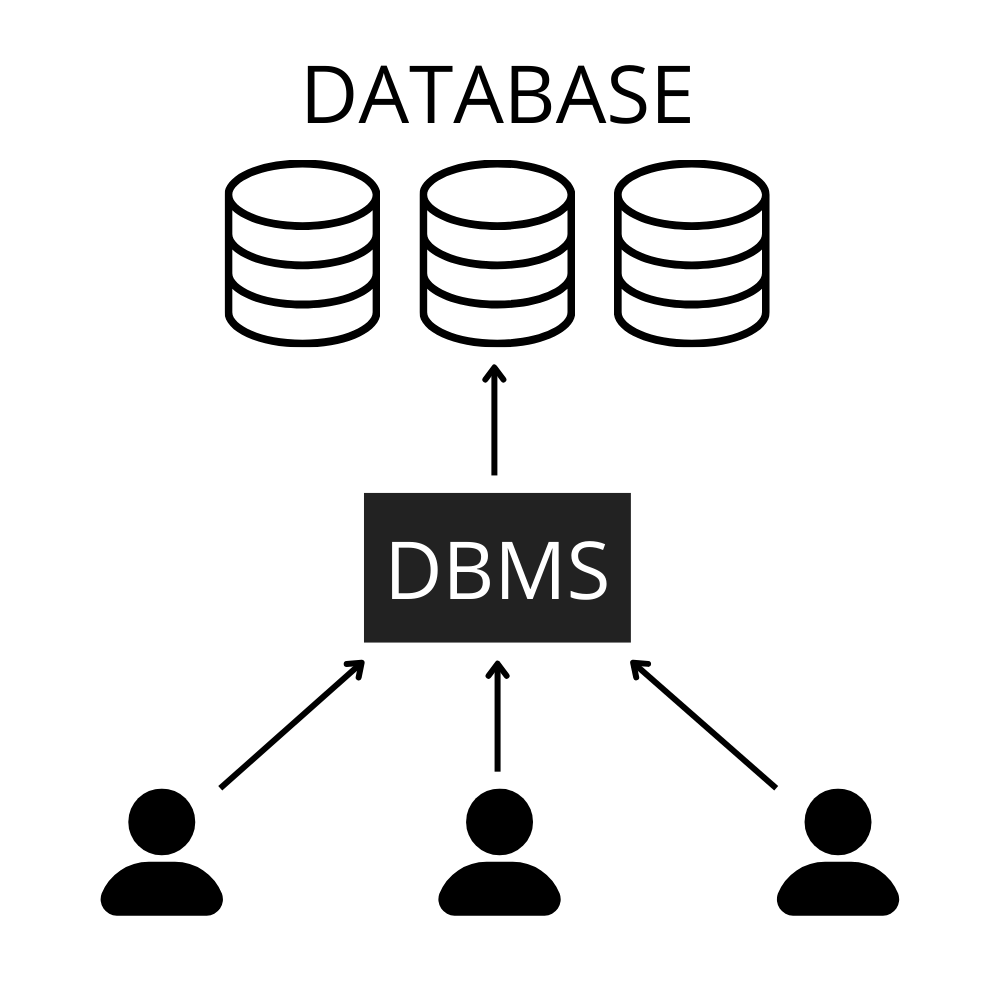
\includegraphics[width=\linewidth]{img/dbms.png}
                \caption{{creata con \href{www.canva.com}{Canva}}}
            \end{figure}
    \end{columns}
\end{frame}

\section{DATABASE RELAZIONALI, PROBLEMI PI\'U COMUNI}

\begin{frame}{PROBLEMI PI\'U COMUNI}
    \begin{alertblock}{RIDONDANZA}
        \begin{minipage}{0.98\linewidth}
            \justifying
            Duplicazione dei dati che provoca un eccessivo e non necessario consumo di memoria.
        \end{minipage}
    \end{alertblock}
    \pause
    \begin{alertblock}{INCONSISTENZA}
        \begin{minipage}{0.98\linewidth}
            \justifying
            Duplicazione di uno stesso dato con nome o tipo diverso che produce 
            incertezza su quale sia la versione corretta del dato. I dati inconsistenti non 
            sono utilizzabili.
        \end{minipage}
    \end{alertblock}
    \pause
    \begin{alertblock}{INCONGRUENZA}
        \begin{minipage}{0.98\linewidth}
            \justifying
            I valori assegnati ai dati non corrispondono al corretto significato degli stessi.
        \end{minipage}
    \end{alertblock}
\end{frame}

\section{DATABASE RELAZIONALI, PROPRIET\'A DA GARANTIRE}

\begin{frame}{PROPRIET\'A DA GARANTIRE}
    \begin{alertblock}{CORRELAZIONE}
        \begin{minipage}{0.98\linewidth}
            \justifying
            I dati sono collegati logicamente da relazioni per evitare la loro duplicazione 
            in archivi diversi.
        \end{minipage}
    \end{alertblock}
    \pause
    \begin{alertblock}{CONDIVISIBILIT\'A}
        \begin{minipage}{0.98\linewidth}
            \justifying
            I dati sono accessibili da utenti diversi secondo le necessità di utilizzo; ogni 
            utente deve poter accedere solo alla parte che gli interessa della base di 
            dati, senza l’obbligo di accedere alla totalità dei dati; i dati sono anche fruibili 
            da applicazioni diverse nello stesso momento.
        \end{minipage}
    \end{alertblock}
    \pause
    \begin{alertblock}{SICUREZZA}
        \begin{minipage}{0.98\linewidth}
            \justifying
            Poiché i dati sono utilizzabili da utenti diversi, è necessario che sia
            predisposto un meccanismo di protezione da interventi non autorizzati o da
            eventi accidentali non dovuti all’intervento umano che possono causare
            perdite di dati, come per esempio un blackout.
        \end{minipage}
    \end{alertblock}
\end{frame}

\begin{frame}{PROPRIET\'A DA GARANTIRE}
    \begin{alertblock}{INTEGRIT\'A}
        \begin{minipage}{0.98\linewidth}
            \justifying
            La base di dati deve garantire l’accesso agli utenti autorizzati, ma deve
            anche essere in grado di proteggere i dati da eventi accidentali causati dalle
            applicazioni (errori di sistema) o dagli utenti stessi (per inesperienza o
            fatalità) che possono produrre inconsistenza dei dati.
        \end{minipage}
    \end{alertblock}
    \pause
    \begin{alertblock}{ELIMINAZIONE DELLA RIDONDANZA}
        \begin{minipage}{0.98\linewidth}
            \justifying
            La base di dati non deve presentare lo stesso dato in archivi diversi o dati 
            simili che permettano di ricavare le stesse informazioni.
        \end{minipage}
    \end{alertblock}
\end{frame}

\begin{frame}{PROPRIET\'A DA GARANTIRE}
    \begin{alertblock}{CONSISTENZA}
        \begin{minipage}{0.98\linewidth}
            \justifying
            I dati devono essere affidabili e reali, quindi non è possibile avere lo stesso
            dato con valori diversi in archivi diversi, inoltre l'aggiornamento degli stessi
            deve avvenire in tempo reale per evitare che operazioni successive
            agiscano su dati non effettivi.
        \end{minipage}
    \end{alertblock}
    \pause
    \begin{alertblock}{PERMANENZA}
        \begin{minipage}{0.98\linewidth}
            \justifying
            La memorizzazione dei dati è effettuata sulla memoria di massa in modo che
            questi siano conservati nel tempo; la loro eliminazione deve avvenire solo
            per volontà del gestore del sistema, in base alle esigenze degli utenti e della
            realtà informatizzata.
        \end{minipage}
    \end{alertblock}
\end{frame}

\section{PROGETTARE UNA BASE DI DATI}

\begin{frame}{PROGETTARE UNA BASE DI DATI}
    \begin{alertblock}{LE TRE FASI DELLA PROGETTAZIONE}
        \begin{minipage}{0.98\linewidth}
            \justifying
            La struttura di una base di dati si crea in funzione delle specifiche esigenze
            aziendali e pertanto il punto di partenza è un’attenta attività di studio e analisi
            della realtà da considerare, che consentirà di ottenere un prodotto da
            verificare ed eventualmente rimodellare per raggiungere la situazione ideale.\\
            \pause
            Le fasi di progettazione sono tre:
            \begin{enumerate}
                \item \textbf{progettazione concettuale};
                \item \textbf{progettazione logica};
                \item \textbf{progettazione fisica}. 
            \end{enumerate}
        \end{minipage}
    \end{alertblock}
\end{frame}

\begin{frame}{PROGETTARE UNA BASE DI DATI}
    \begin{columns}
        \column{.7\textwidth}
            \begin{alertblock}{PROGETTAZIONE CONCETTUALE}
                \begin{minipage}{0.98\linewidth}
                    \justifying
                    La progettazione concettuale consiste nell’analisi della realtà, per raccogliere
                    le informazioni utili da informatizzare in base alle necessità degli utenti che le
                    dovranno utilizzare. Questa prima fase non tiene in considerazione la
                    tecnologia e produce uno schema formale e completo con tutti i dati necessari
                    e le relazioni che li correlano. Questo livello di progettazione si definisce
                    esterno perché indipendente dagli aspetti informatici del problema.\\
                    \textbf{Per realizzare lo schema concettuale si utilizza il modello entità-relazione (E/R).}
                \end{minipage}
            \end{alertblock}
        \column{.3\textwidth}
            \begin{figure}
                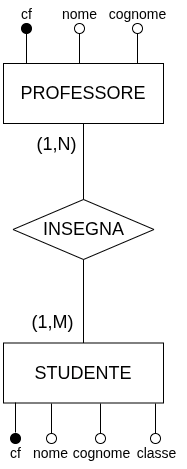
\includegraphics[width=.6\linewidth]{img/esempioER.png}
                \caption{{creata con \href{https://app.diagrams.net/}{Diagrams.net}}}
            \end{figure}
    \end{columns}
\end{frame}

\begin{frame}{PROGETTARE UNA BASE DI DATI}
    \begin{columns}
        \column{.6\textwidth}
            \begin{alertblock}{PROGETTAZIONE LOGICA}
                \begin{minipage}{0.98\linewidth}
                    \justifying
                    La progettazione logica consiste nel definire uno schema logico dei dati in
                    base alle tecnologie informatiche che si hanno a disposizione; lo schema
                    logico si crea partendo dal modello concettuale ideato nella fase precedente e
                    permette di specificare le relazioni ipotizzate. Questo livello si chiama logico
                    perché definisce le strutture astratte che contengono i dati necessari per
                    l’elaborazione delle informazioni.\\
                    \textbf{Traduzione del modello entità-relazione (E/R) nelle effettive tabelle che 
                    compongono il database.}
                \end{minipage}
            \end{alertblock}
        \column{.4\textwidth}
            \begin{figure}
                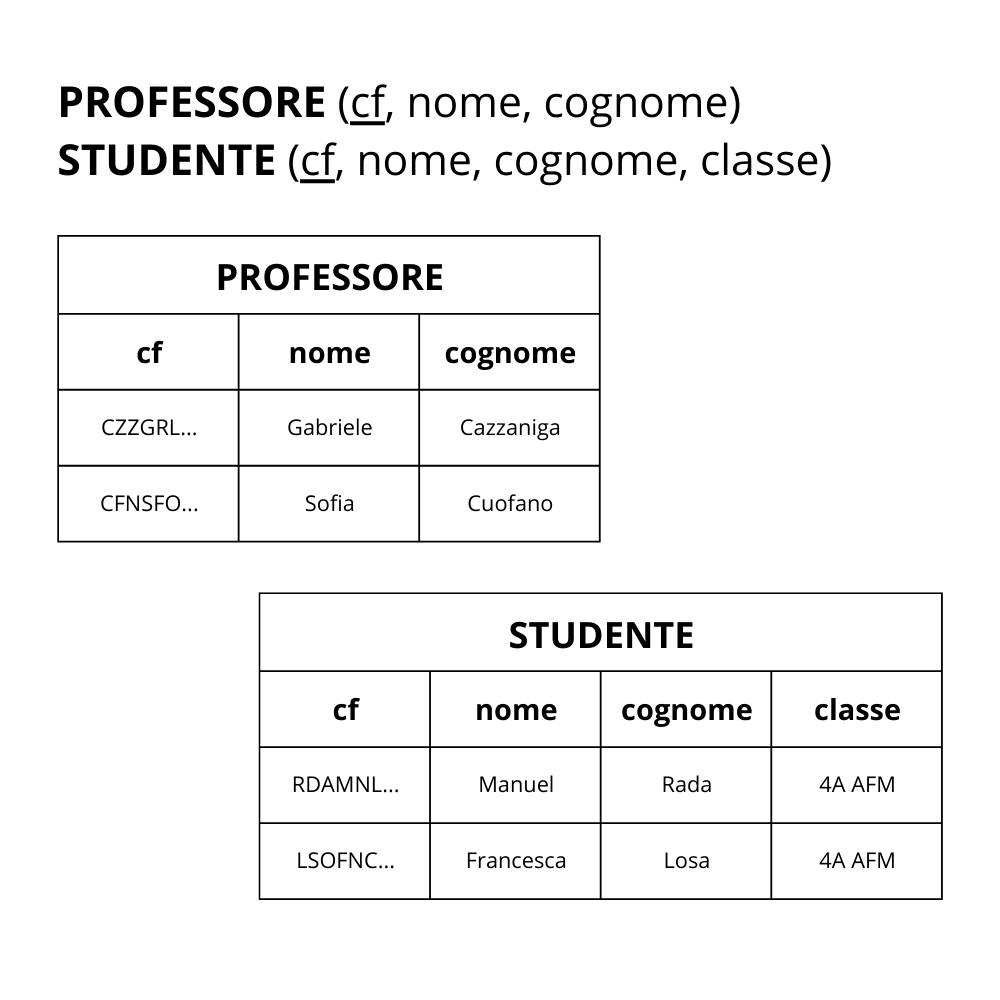
\includegraphics[width=\linewidth]{img/esempioLogico.png}
                \caption{{creata con \href{www.canva.com}{Canva}}}
            \end{figure}
    \end{columns}
\end{frame}

\begin{frame}{PROGETTARE UNA BASE DI DATI}
    \begin{alertblock}{PROGETTAZIONE FISICA}
        \begin{minipage}{0.98\linewidth}
            \justifying
            La progettazione fisica consiste nell’implementazione in memoria di massa dei
            dati e delle loro relazioni definiti nel livello precedente; il risultato consiste
            nella memorizzazione su disco dei dati descritti. Questo livello si definisce
            fisico perché vengono organizzate le strutture concrete che conterranno i dati.\\
            \textbf{Implementazione del modello logico tramite l’utilizzo di un software 
            DBMS (Database Management System).}
        \end{minipage}
    \end{alertblock}
\end{frame}

\end{document}